% TODO: Add a picture of each project here
\section{Proje\textcolor{mycolor}{cts}}
  \subsection{TOS GNU/linux}
    My own Linux distribution based on Arch Linux.\footnote{Servers are hosted in Germany, if you are visting from outside the EU, expect high ping and latency.}

    \begin{center}
      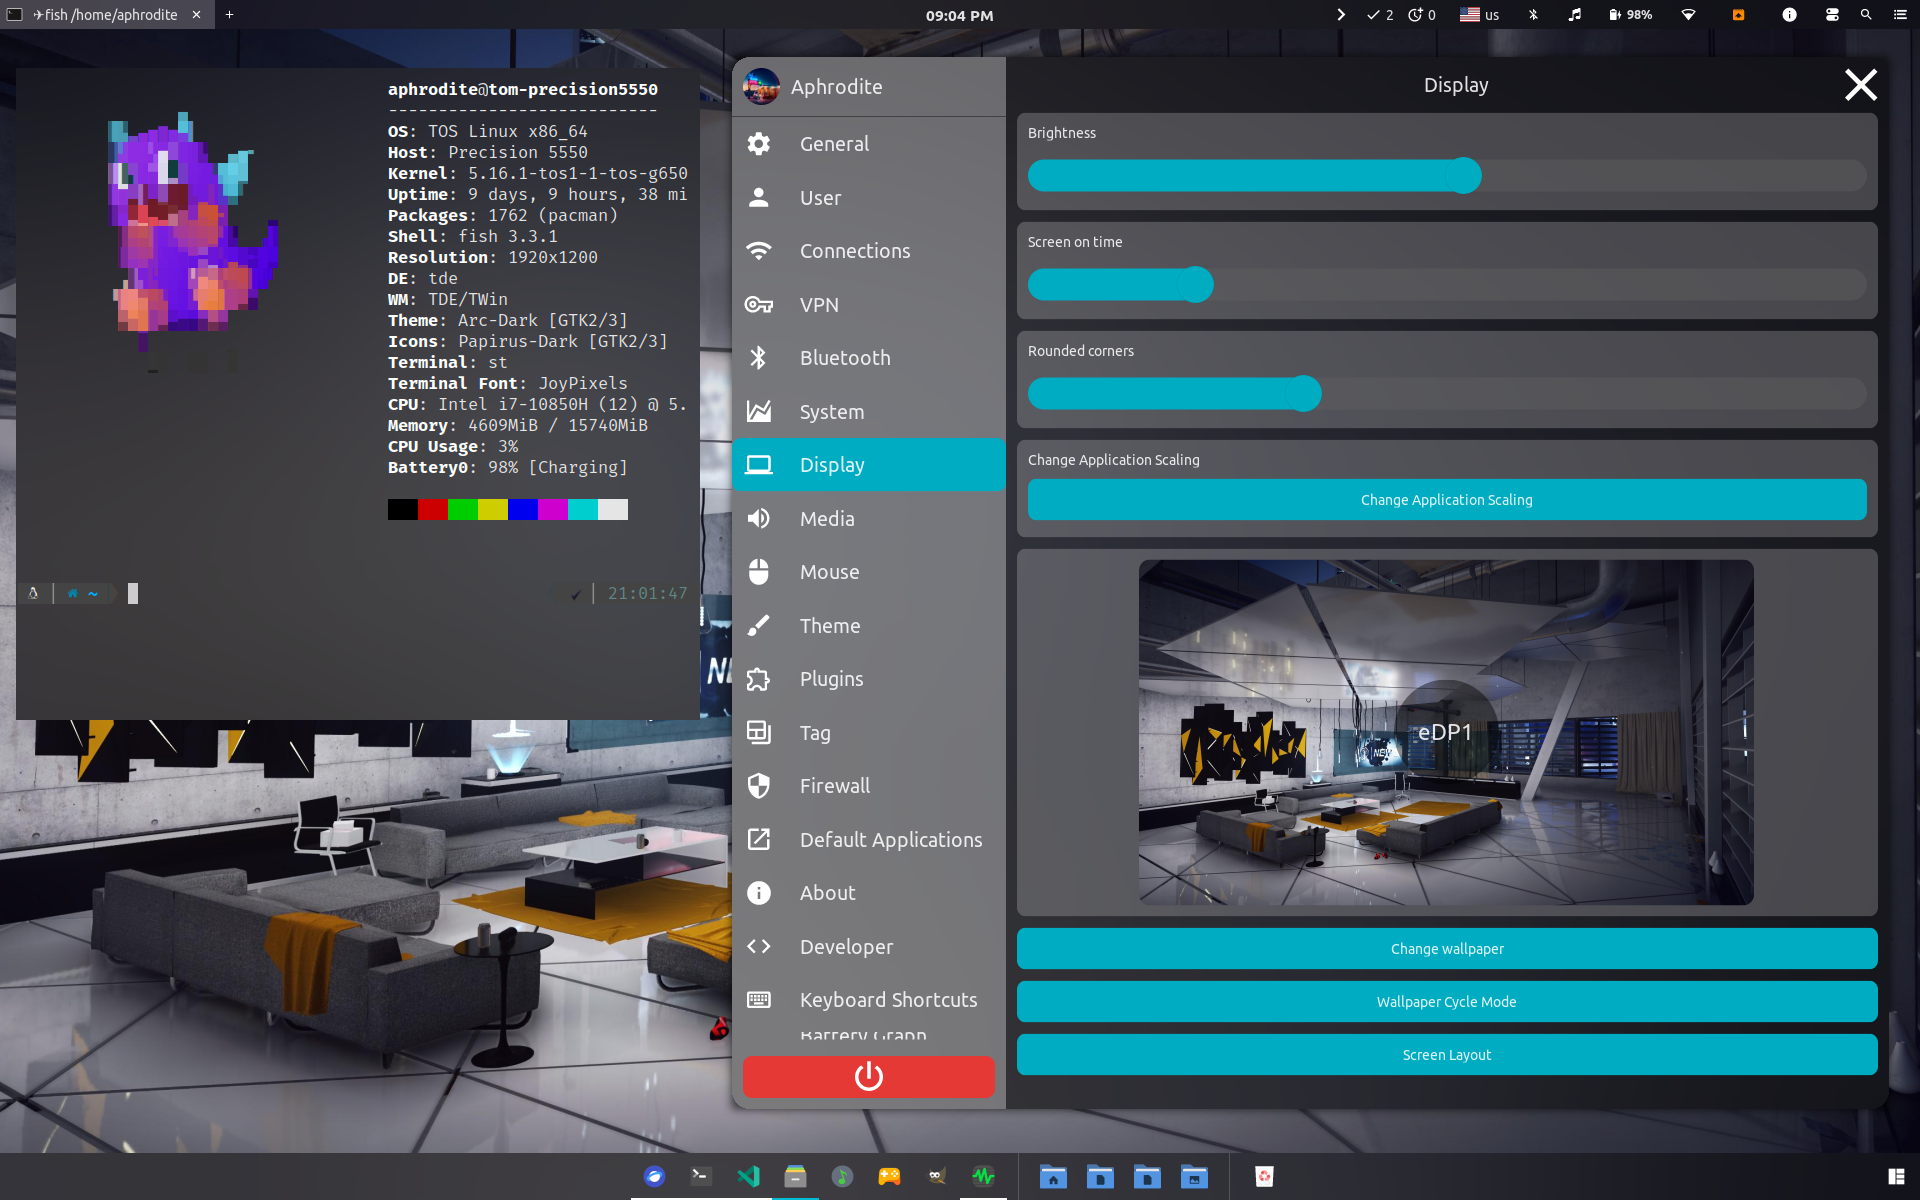
\includegraphics[width=0.7\textwidth]{desktop}
    \end{center}

    \subsubsection{Live Iso}
      You can try the live iso \href{https://tos.odex.be}{here}.\footnotemark[\value{footnote}]
    \subsubsection{Repository}
      TOS Hosts its own packages and Linux kernel \href{https://repo.odex.be/list.html}{here}.\footnotemark[\value{footnote}]
    \subsubsection{Duration}
      3 years and ongoing.

\pagebreak

  \subsection{Automated Paintball gun}
    Scan for movement and automatically move the gun there to shoot the target.
    The goal of this project is to assist when going to paintball,
    it will detect movement from the 'enemy' team and start shooting paintball's there.
    \begin{center}
      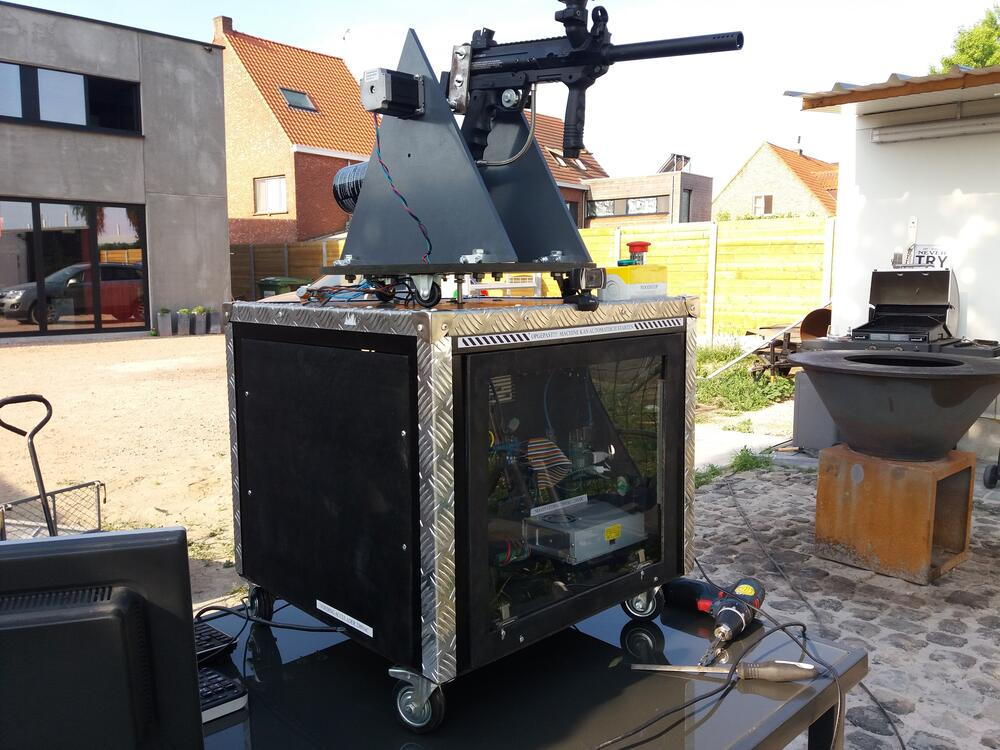
\includegraphics[width=0.7\textwidth]{paintball}
    \end{center}
    \subsubsection{Duration}
      1 year.

\vspace{2cm}

  \subsection{3D First Person Shooter}
    Operation Red Dragon is a 3D first person shooter with realistic graphics available on Steam.
    \begin{center}
      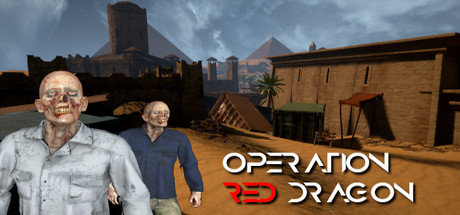
\includegraphics[width=0.7\textwidth]{game}
    \end{center}
    \subsubsection{Steam Page}
      For more information about the game visit \href{https://store.steampowered.com/app/747730/Operation_Red_Dragon/}{here}.